\documentclass{article}

\usepackage{graphicx}
\usepackage{tikz}
\usepackage{tikzsymbols}
\usetikzlibrary{calc,patterns,shapes.geometric}
\pagestyle{empty}
\usepackage[margin=0pt]{geometry}
\geometry{papersize={14in,12in}}

\def\centerarc[#1](#2)(#3:#4:#5){\draw[#1] ($(#2)+({#5*cos(#3)},{#5*sin(#3)})$) arc (#3:#4:#5);}

\begin{document}
	\begin{figure}
		\centering
		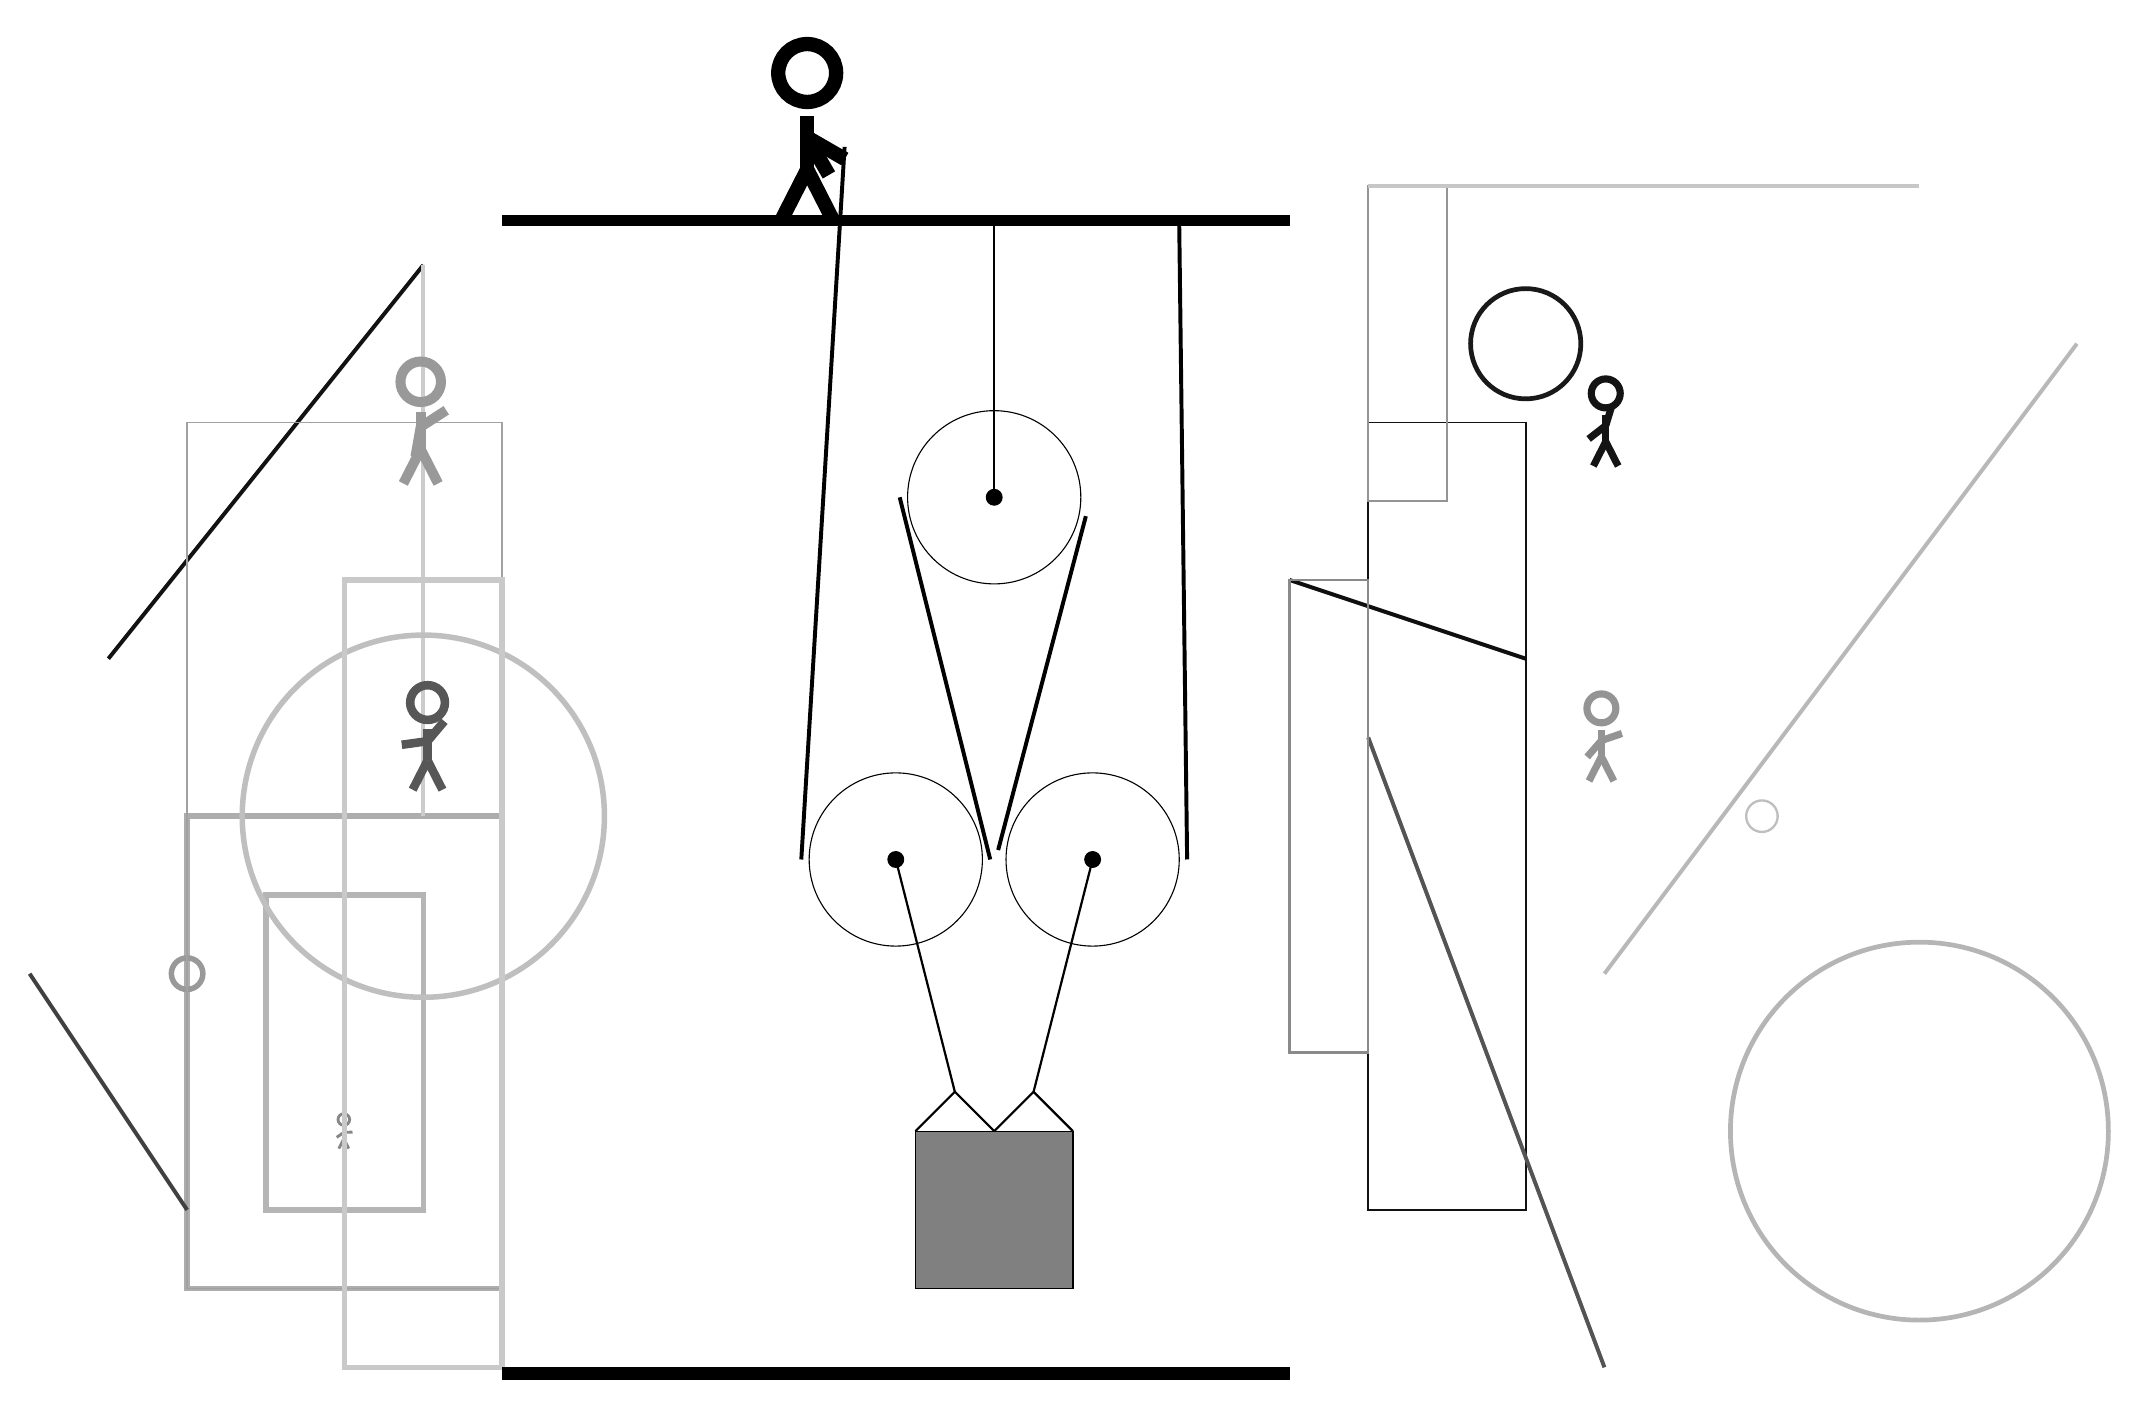
\begin{tikzpicture}
			%%%%% START %%%%%
			
			\draw[fill=black] (-4, 11.5) rectangle (6, 11.625);
			
			\draw (1, 3.45) circle (1.1);
			\draw[fill=black] (1, 3.45) circle (0.1);
			
			\draw (2.25, 8.05) circle (1.1);
			\draw[fill=black] (2.25, 8.05) circle (0.1);
			\draw[thick] (2.25, 8.05) -- (2.25, 11.5);
			
			\draw (3.5, 3.45) circle (1.1);
			\draw[fill=black] (3.5, 3.45) circle (0.1);
			
			\draw[thick] (3.5, 3.45) -- (2.75, 0.5);
			\draw[thick] (1, 3.45) -- (1.75, 0.5);
			\draw[thick]  (1.25, 0) -- (1.75, 0.5) -- (2.25, 0);
			\draw[thick]  (2.25, 0) -- (2.75, 0.5) -- (3.25, 0);
			\draw[fill=black!50] (1.25, 0) rectangle (3.25, -2);
			
			\draw[line width=0.2mm, color=black!93] (7, -1) rectangle (9, 9);
			
			\node[line width=0.4mm, color=black!47] at (-6, 0) {\Strichmaxerl[2][35][2]};
			\draw[line width=0.7mm, color=black!32] (-4, 4) rectangle (-8, -2);
			\draw[line width=0.5mm, color=black!28](10, 2) -- (16, 10);
			\draw[line width=0.5mm, color=black!93](-9, 6) -- (-5, 11);
			
			\draw[line width=0.5mm, color=black!20] (-5, 11) rectangle (-5, 4);
			\node[line width=0.2mm, color=black!92] at (10, 9) {\Strichmaxerl[5][38][73]};
			
			\node[line width=0.6mm, color=black!66] at (-5, 5) {\Strichmaxerl[6][8][50]};
			\draw[line width=0.7mm, color=black!29] (-5, -1) rectangle (-7, 3);
			\draw [line width=0.6mm, color=black!90](9, 10) circle (0.7);
			\draw [line width=0.6mm, color=black!29](14, 0) circle (2.4);
			
			\draw [line width=0.3mm, color=black!25](12, 4) circle (0.2);
			\draw[line width=0.5mm, color=black!94](6, 7) -- (9, 6);
			
			\draw [line width=0.7mm, color=black!40](-8, 2) circle (0.2);
			\draw[line width=0.3mm, color=black!42] (7, 8) rectangle (8, 12);
			\draw [line width=0.7mm, color=black!25](-5, 4) circle (2.3);
			
			\draw[line width=0.5mm, color=black!67](10, -3) -- (7, 5);
			
			\draw[line width=0.2mm, color=black!37] (-4, 9) rectangle (-8, -2);
			\draw[line width=0.3mm, color=black!46] (6, 1) rectangle (7, 7);
			\node[line width=0.3mm, color=black!40] at (-5, 9) {\Strichmaxerl[7][80][33]};
			\draw[line width=0.5mm, color=black!75](-8, -1) -- (-10, 2);
			
			\draw[line width=0.5mm, color=black!22](7, 12) -- (14, 12);
			\draw[line width=0.7mm, color=black!21] (-4, 7) rectangle (-6, -3);
			\node[line width=0.3mm, color=black!42] at (10, 5) {\Strichmaxerl[5][49][19]};
			
			\draw[line width=0.5mm] (0.35, 12.5) --  (-0.2, 3.45);
			\centerarc[line width=0.5mm](1, 3.45)(180:360:1.2000000000000002);
			\draw[line width=0.5mm] (2.2, 3.45) -- (1.05, 8.05);
			\centerarc[line width=0.5mm](2.25, 8.05)(-20:180:1.2000000000000002);
			\draw[line width=0.5mm](3.414, 7.81) -- (2.3, 3.57);
			\centerarc[line width=0.5mm](3.5, 3.45)(160:360:1.2000000000000002);
			\draw[line width=0.5mm](4.7, 3.45) -- (4.6, 11.5);
			
			\node at (-0.07, 12.7) {\Strichmaxerl[10][120][-30]};
			
			\draw[fill=black] (-4, -3) rectangle (6, -3.15);
			
			%%%%% END %%%%%
		\end{tikzpicture}
	\end{figure}	
\end{document}